% \documentclass{standalone}

% \input{../tikz_header}

% \begin{document}


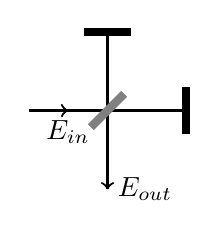
\begin{tikzpicture}[BS style/.style={draw=gray, line width=3pt},
    mirror style/.style={draw=black, line width=3pt},]
    %\useasboundingbox (-2.5,-1.5) rectangle (3,2.3);
    %\draw (-2.5,-1.5) rectangle (3,2.3);
 
    \pgfmathsetmacro{\len}{0.3}


    \coordinate (BS) at (0,0);
    \coordinate (m1) at (1,0);
    \coordinate (m2) at (0,1);
    \coordinate (in) at (-1,0);
    \coordinate (out) at (0,-1);

    \draw[thick] (in) -- (m1);
    \draw[thick, -> ] (in) -- ++(0:0.5) node[below] {$E_{in}$};
    \draw[thick] (out) -- (m2);
    \draw[thick, <- ] (out) node[right] {$E_{out}$} -- ++(90:0.5);


    \draw[style=BS style] (BS) ++ (45:\len) -- ++(-135:{2*\len});
    \draw[style=mirror style] (m2) ++ (180:\len) -- ++(0:{2*\len});
    \draw[style=mirror style] (m1) ++ (90:\len) -- ++(-90:{2*\len});
   


\end{tikzpicture}


%\end{document}